\chapter{Dataset}

This study focuses exclusively on firms listed in United States equity markets. 
The U.S. market was selected for three principal reasons. 
First, it is the largest and most liquid equity market globally, providing a rich cross-section of firms across sectors and industries. 
Second, U.S. disclosure requirements are among the most stringent and standardized worldwide, ensuring high-quality, comparable corporate reporting. 
Third, the availability of structured financial, textual, and market data is substantially greater than in most international markets, making it particularly well-suited for large-scale empirical and machine learning research.

\section{SEC Filings}

Corporate disclosure in the United States is regulated by the U.S. Securities and Exchange Commission (SEC), which requires publicly traded firms to submit periodic filings through the Electronic Data Gathering, Analysis, and Retrieval (EDGAR) system. 
These filings serve as primary sources of information for investors, analysts, and regulators.

Among the wide range of SEC forms, this study focuses exclusively on Form 10-K and Form 10-Q. 
The 10-K is the firm's annual report, providing a comprehensive overview of financial performance, business operations, risk factors, and management analysis for the fiscal year. 
The 10-Q is the corresponding quarterly report, offering interim updates on financial condition and results of operations.
Together, these two forms represent the most detailed and standardized recurring disclosures made by U.S. public companies.

The choice to restrict attention to 10-K and 10-Q filings is motivated by their informational richness and regulatory consistency. 
Unlike event-driven filings (e.g., 8-K) that may be triggered by heterogeneous corporate events, 10-K and 10-Q reports are mandatory, regularly scheduled disclosures that follow standardized content requirements. 
Prior research demonstrates that these filings contain economically meaningful information relevant to valuation and risk assessment\cite{textual-analysis-dictionaries-and-10ks}. 
Focusing on these forms ensures comparability across firms and time, while concentrating on disclosures that are central to investors' expectations formation.

The textual data were obtained from the University of Notre Dame's cleaned \href{https://sraf.nd.edu/sec-edgar-data/}{SEC filings dataset}, which removes HTML tags, tables, and formatting artifacts from raw EDGAR documents. 
This preprocessing is particularly important for natural language processing applications, as raw filings often contain extensive markup and tabular structures that are not directly usable in textual modeling.

The sample period spans 2011 to 2024. 
The starting point was selected to reflect modern market conditions and reporting practices. 
Following regulatory changes such as the adoption of XBRL (eXtensible Business Reporting Language) requirements in the late 2000s and early 2010s, SEC filings became more standardized and machine-readable. 
The SEC mandated phased XBRL adoption beginning in 2009, with full compliance across firms in the early 2010s, substantially increasing structural consistency in filings. 
Restricting the sample to 2011 onward therefore improves comparability and alignment with contemporary disclosure formats. 
Additionally, older financial data may reflect structural market conditions, such as lower algorithmic trading penetration and different regulatory environments, that are less representative of today's market microstructure.

\subsection{Section Extraction and Text Processing}

Although 10-K and 10-Q filings are information-rich, they are also lengthy and heterogeneous.
Not all sections are equally relevant for short-term stock price prediction. 
Therefore, rather than using the entire filing, this study focuses on two specific sections: 
Management's Discussion and Analysis of Financial Condition and Results of Operations (MD\&A) and Quantitative and Qualitative Disclosures About Market Risk.

The MD\&A section provides management's narrative explanation of financial performance, liquidity, capital resources, and operational trends. 
It frequently includes forward-looking statements, explanations of earnings changes, and contextual discussion that goes beyond raw financial statements. 
Prior literature highlights the importance of textual tone and narrative disclosures in influencing investor reactions.

The “Quantitative and Qualitative Disclosures About Market Risk” section addresses exposures to interest rate risk, currency risk, commodity price risk, and other financial uncertainties. 
These disclosures are directly relevant to risk assessment and may influence investors' expectations about future volatility and firm performance.

Section extraction was performed using regular expression matching to isolate these components from each filing. 
Because automated extraction may occasionally fail or capture unintended content, additional filtering steps were applied. 
Very short lines and lines without alphabetic characters were removed, as these often correspond to residual table fragments or formatting artifacts rather than meaningful narrative text. 
Samples with total character counts exceeding the 99th percentile were excluded, as these typically reflected extraction errors. 
Filings with fewer than two lines of extracted text, or with both targeted sections empty, were also removed to ensure substantive textual content.

These preprocessing decisions aim to balance textual richness with data quality, ensuring that the resulting corpus is both economically meaningful and suitable for NLP-based modeling.

\subsection{Manual Quality Inspection}

After applying the cleaning and preprocessing pipeline described in the previous section, the dataset contained more than 350,000 extracted section texts. Given the scale of the corpus, manually inspecting every observation was infeasible. Instead, we performed a structured random quality check by sampling 30 observations from each section (MD\&A and Market Risk) and inspecting them manually.

This sampling-based validation procedure is common in large-scale text mining research, where exhaustive manual verification is impractical. Random inspection of a sufficiently large subset provides a statistically reasonable assessment of extraction quality, especially when the extraction process follows deterministic rules. Such spot checks are widely used in information retrieval and natural language processing pipelines to ensure that automated extraction procedures do not introduce systematic noise.

During the inspection, we verified that:
\begin{itemize}
    \item The extracted text corresponded to the intended section headers.
    \item The text did not include substantial spillover from adjacent sections.
    \item The preprocessing pipeline did not remove excessive content.
    \item The remaining text contained economically meaningful information.
\end{itemize}

The inspection indicated that the extraction procedure performed reliably and that the preprocessing step preserved the substantive content of the filings.

\subsection*{Missing Sections}

A section is considered missing if the extracted text is an empty string. Missingness may arise for multiple reasons:
\begin{itemize}
    \item Failure of the extraction rule to detect the section.
    \item Filings in which the section is intentionally omitted.
    \item Cases where the filing refers to another document (e.g., incorporation by reference).
    \item Sections deemed too short and removed during preprocessing.
\end{itemize}

Across the full sample, the MD\&A section is missing in 1.77\% of filings, whereas the Market Risk section is missing in 73.29\% of filings. The substantially higher missing rate for Market Risk reflects structural differences between filing types, as certain forms do not systematically contain a standalone market risk discussion.

Because of this asymmetry, we concatenate the MD\&A and Market Risk sections prior to sentiment extraction. This ensures that sentiment signals are captured even when one of the sections is absent.

\begin{figure}[H]
    \centering
    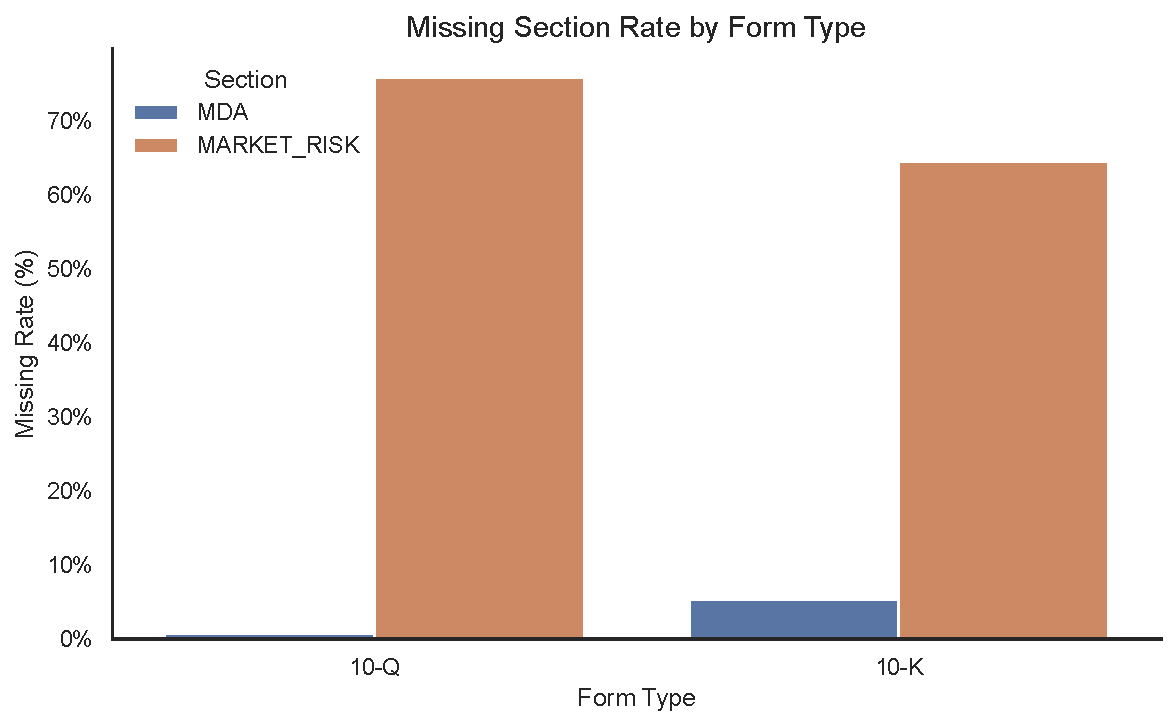
\includegraphics[width=0.75\linewidth]{sec_filings_images/missing_rate_by_form_type.pdf}
    \caption{Missing rate of MD\&A and Market Risk sections by form type (10-K and 10-Q).}
    \label{fig:missing_by_form}
\end{figure}

\subsection*{Text Length Statistics}

We next examine the statistical properties of the extracted sections based on character count. Observations with zero-length text were excluded from this analysis, as they correspond to missing extractions rather than valid textual content.

\subsubsection*{MD\&A Section}

The MD\&A section is substantially longer and more variable than the Market Risk section:

\begin{itemize}
    \item Mean length: 42,589 characters
    \item Standard deviation: 33,575
    \item Minimum: 2,000
    \item 10th percentile: 10,172
    \item 25th percentile: 19,117
    \item Median: 35,105
    \item 75th percentile: 55,586
    \item 90th percentile: 81,916
    \item Maximum: 235,166
\end{itemize}

These statistics indicate a highly dispersed and right-skewed distribution. While the median filing contains approximately 35,000 characters, the upper tail extends beyond 200,000 characters, reflecting considerable heterogeneity in disclosure practices.

\subsubsection*{Market Risk Section}

The Market Risk section is significantly shorter:

\begin{itemize}
    \item Mean length: 6,893 characters
    \item Standard deviation: 8,986
    \item Minimum: 2,000
    \item 10th percentile: 2,322
    \item 25th percentile: 2,891
    \item Median: 4,125
    \item 75th percentile: 6,666
    \item 90th percentile: 12,613
    \item Maximum: 71,860
\end{itemize}

Although shorter on average, the Market Risk section also exhibits right-skewness, with a small number of filings containing extensive risk disclosures.

To visualize the distribution of text lengths, we employ a logarithmic scale. This is necessary because SEC filings exhibit heavy-tailed behavior: a small number of extremely long filings would compress the majority of observations near zero on a linear scale. A logarithmic transformation provides a clearer representation of the underlying distributional shape and dispersion.

Filings with zero-length sections were excluded from these plots, as they represent missing extractions rather than valid text.

\begin{figure}[H]
    \centering
    \begin{minipage}{0.48\linewidth}
        \centering
        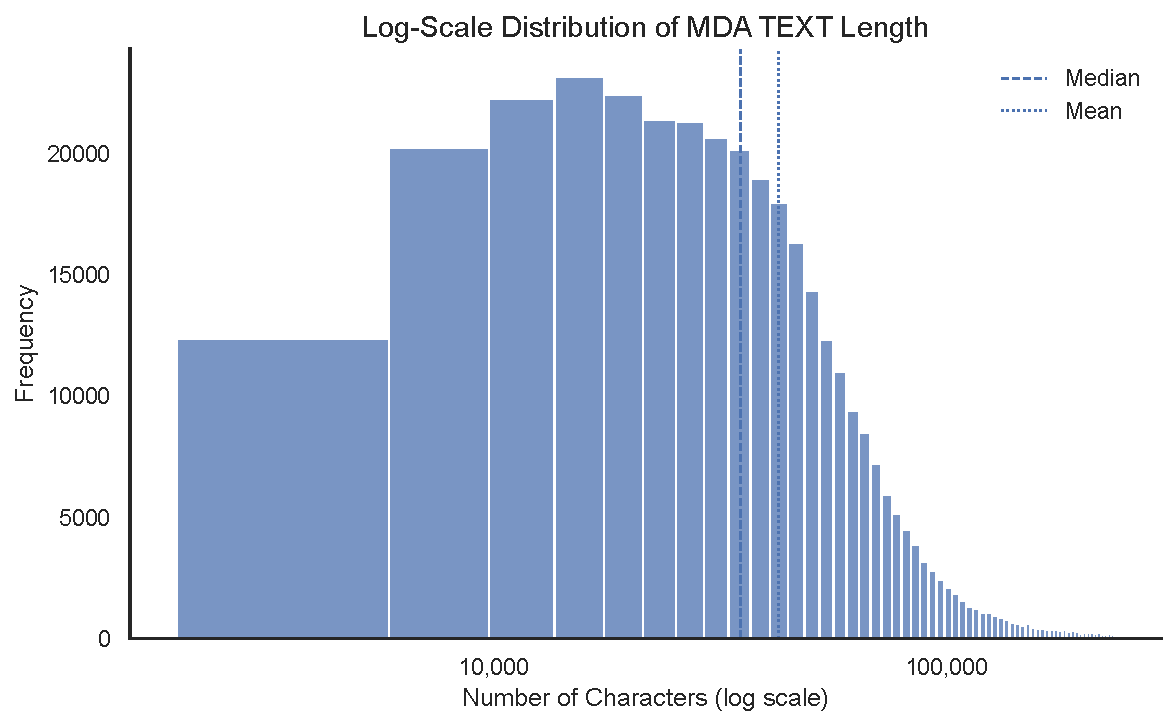
\includegraphics[width=\linewidth]{sec_filings_images/mda_text_length_distribution_log.pdf}
        \caption*{(a) MD\&A}
    \end{minipage}
    \hfill
    \begin{minipage}{0.48\linewidth}
        \centering
        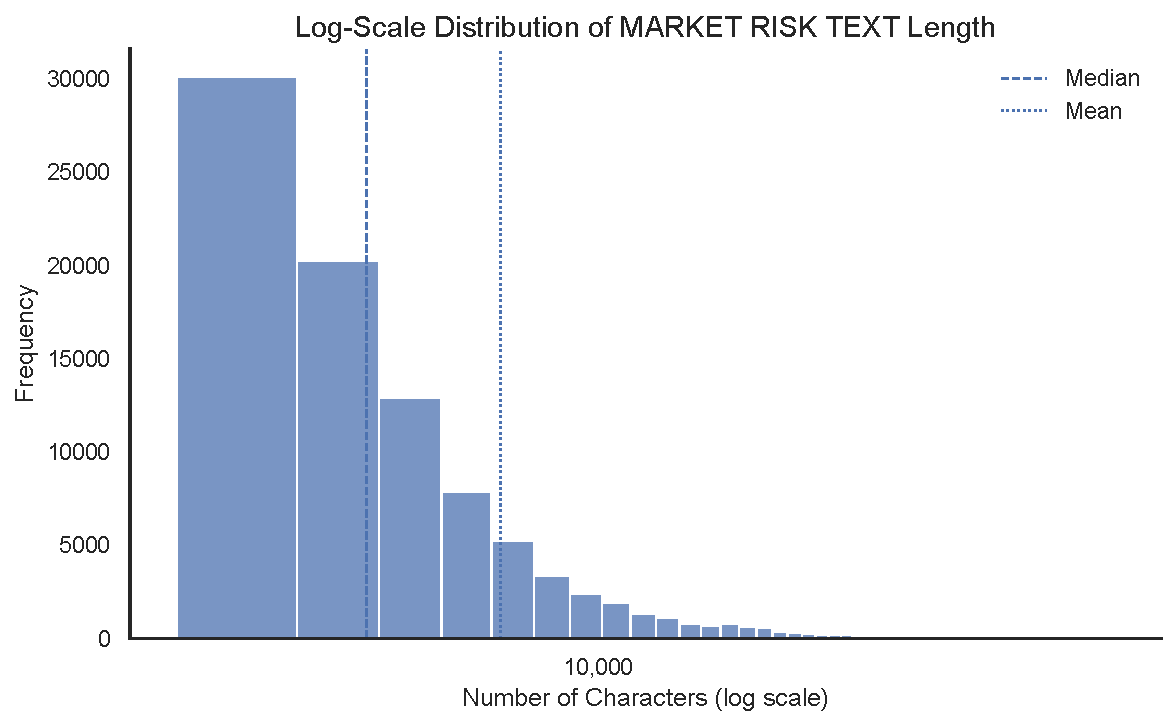
\includegraphics[width=\linewidth]{sec_filings_images/market_risk_text_length_distribution_log.pdf}
        \caption*{(b) Market Risk}
    \end{minipage}
    \caption{Log-scale distribution of section lengths (character count).}
    \label{fig:length_distributions}
\end{figure}

Finally, we examine the temporal distribution of filings. The number of SEC filings per year remains relatively stable throughout the sample period. The highest number of filings occurs in 2011, followed by a gradual and moderate decline toward 2024. The overall stability suggests that the dataset does not suffer from severe temporal imbalance, which is important for downstream modeling tasks.

\begin{figure}[H]
    \centering
    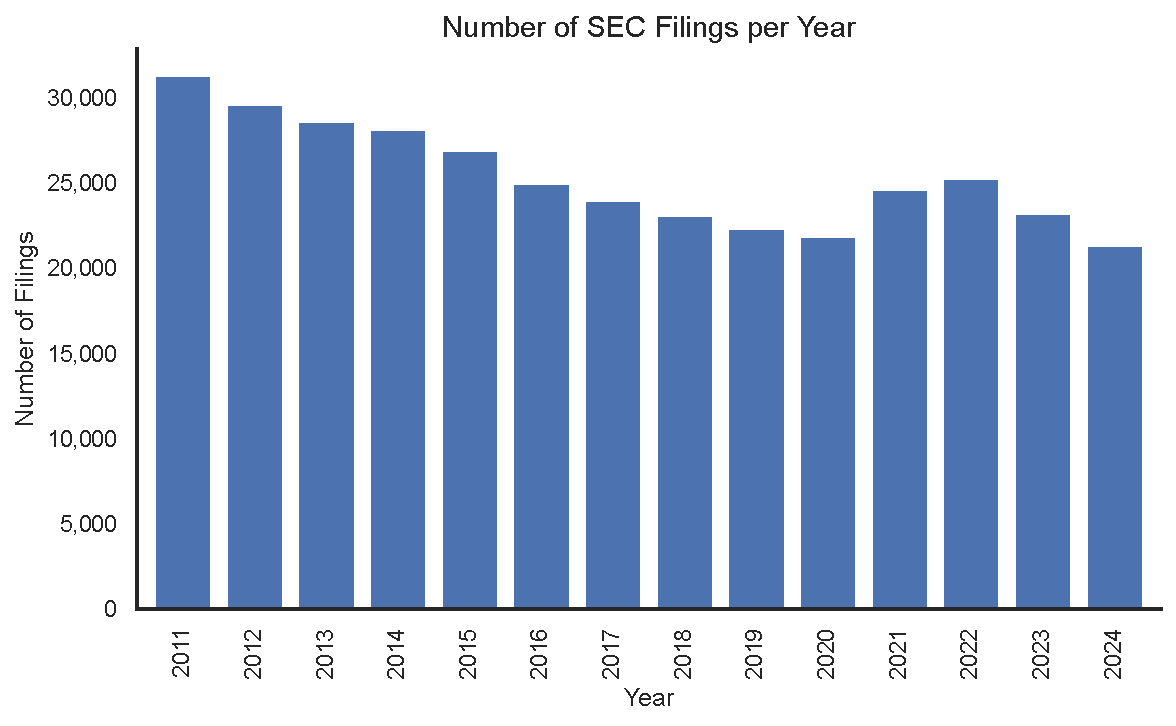
\includegraphics[width=0.75\linewidth]{sec_filings_images/filings_per_year_distribution.pdf}
    \caption{Number of SEC filings per year.}
    \label{fig:filings_per_year}
\end{figure}

Overall, the exploratory analysis confirms that the extraction procedure yields economically meaningful text, that missingness is concentrated primarily in the Market Risk section, and that text length distributions are heavy-tailed and highly heterogeneous. These properties motivate the modeling choices described in subsequent sections, particularly the use of chunk-based processing strategies for long-document sentiment extraction.

\subsection{Firm Identifier Mapping: CIK to Ticker}

The cleaned SEC dataset contains firm identifiers in the form of Central Index Key (CIK) codes assigned by the SEC. 
However, stock price databases typically use ticker symbols. 
To align filings with market data, it was necessary to construct a mapping from CIK to ticker.

This mapping was created by combining two sources. 
First, the SEC's Insider Transactions Data Sets (Forms 3, 4, and 5) were used, as these filings often include both CIK and ticker information. 
These historical submissions provide time-varying mappings that are particularly useful for capturing changes in ticker symbols over time. 
Second, the SEC's publicly available ticker-to-CIK mapping file (\href{https://www.sec.gov/include/ticker.txt}{ticker.txt}) was used to supplement recent mappings. 
Because the latter primarily reflects current ticker assignments and may not accurately represent historical changes, combining both sources improves coverage and historical accuracy.

After mapping CIK identifiers to stock tickers, each ticker is treated as a distinct firm in the dataset. This transformation allows us to move from a filing-level perspective to a firm-level panel structure analysis. The objective of this section is to assess cross-sectional coverage, panel balance, and potential concentration effects that may influence downstream machine learning models.

\subsection*{Overall Firm Coverage}

The final dataset contains 119,613 filings corresponding to 3,671 unique companies. On average, each firm contributes 32.58 filings. This indicates that the dataset has both substantial cross-sectional breadth and meaningful longitudinal depth.

The relatively large number of firms ensures that the dataset captures heterogeneous disclosure behavior across industries and firm sizes. At the same time, the average of roughly 33 filings per firm suggests that many firms are observed repeatedly over time, making the dataset suitable for panel-based empirical analysis and machine learning models that benefit from repeated firm observations.

\subsection*{Distribution of Filings per Company}

Table-level statistics reveal a moderately dispersed distribution of filings per firm:

\begin{itemize}
    \item Median filings per company: 33
    \item 10th percentile: 6
    \item 25th percentile: 14
    \item 75th percentile: 54
    \item 90th percentile: 56
    \item Maximum: 112
\end{itemize}

The median (33) is very close to the mean (32.58), suggesting that the distribution is not heavily skewed. The 10th percentile indicates that even relatively inactive firms contribute multiple filings (at least six), while firms in the upper quartile contribute more than 54 filings. The maximum of 112 filings suggests that some firms are observed across nearly the entire sample period and across multiple filing types.

Figure~\ref{fig:filings_per_company} visualizes the distribution of filings per firm on a logarithmic scale. The log transformation improves interpretability by preventing firms with very high filing counts from visually compressing the majority of observations.

\begin{figure}[H]
    \centering
    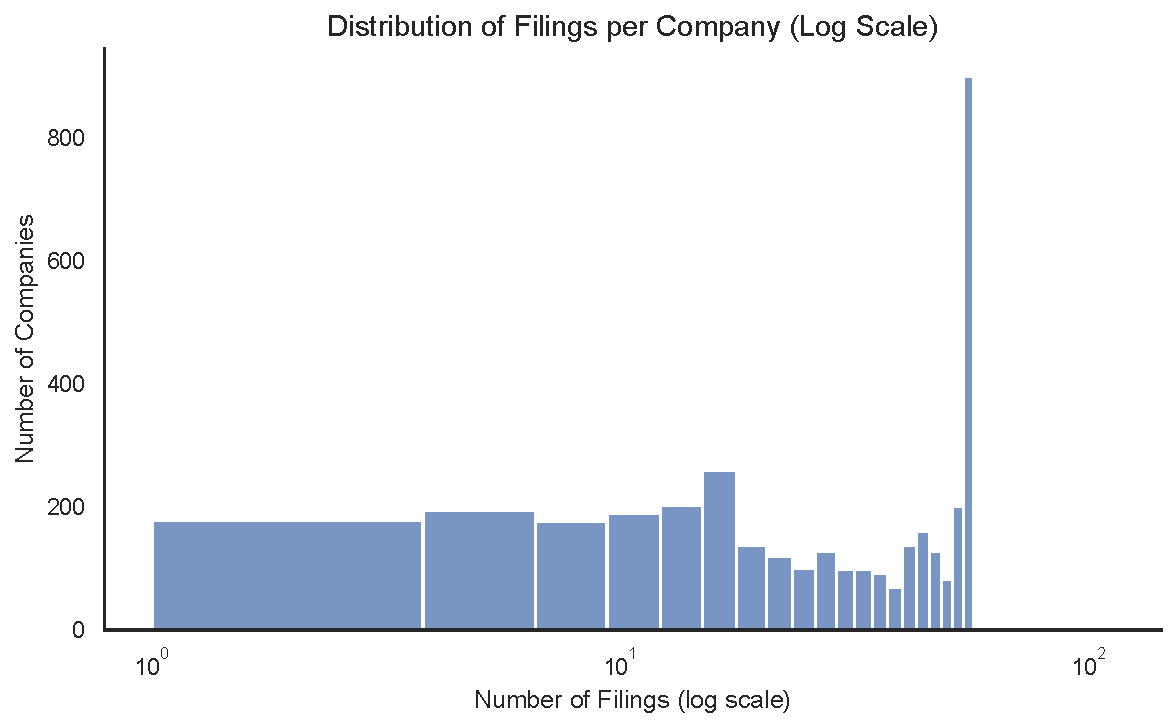
\includegraphics[width=0.75\linewidth]{sec_filings_images/filings_per_company_distribution_log.pdf}
    \caption{Distribution of filings per company (log scale).}
    \label{fig:filings_per_company}
\end{figure}

Overall, the distribution suggests moderate heterogeneity but no extreme dominance by a small number of firms.

\subsection*{Concentration Analysis}

To formally assess whether the dataset is dominated by a small number of highly active firms, we compute filing concentration measures:

\begin{itemize}
    \item Top 1 company share: 0.09\%
    \item Top 5 companies share: 0.39\%
    \item Top 10 companies share: 0.68\%
\end{itemize}

These values indicate very low concentration. Even the ten most active firms together account for less than 1\% of total filings. This is an important property for machine learning applications: the training data is not disproportionately influenced by a handful of firms. Consequently, learned representations are less likely to be biased toward firm-specific disclosure styles of a few dominant entities.

From a statistical perspective, this reduces the risk of overfitting to idiosyncratic firm language patterns and improves the external validity of the trained models.

\subsection*{Time Coverage per Company}

Next, we examine the longitudinal coverage of firms. The median firm is observed for 9.25 years, while firms in the 90th percentile are observed for 13.71 years. The maximum coverage is 13.96 years, which is nearly the full sample period.

Figure~\ref{fig:company_time_coverage} shows the distribution of years covered per firm.

\begin{figure}[H]
    \centering
    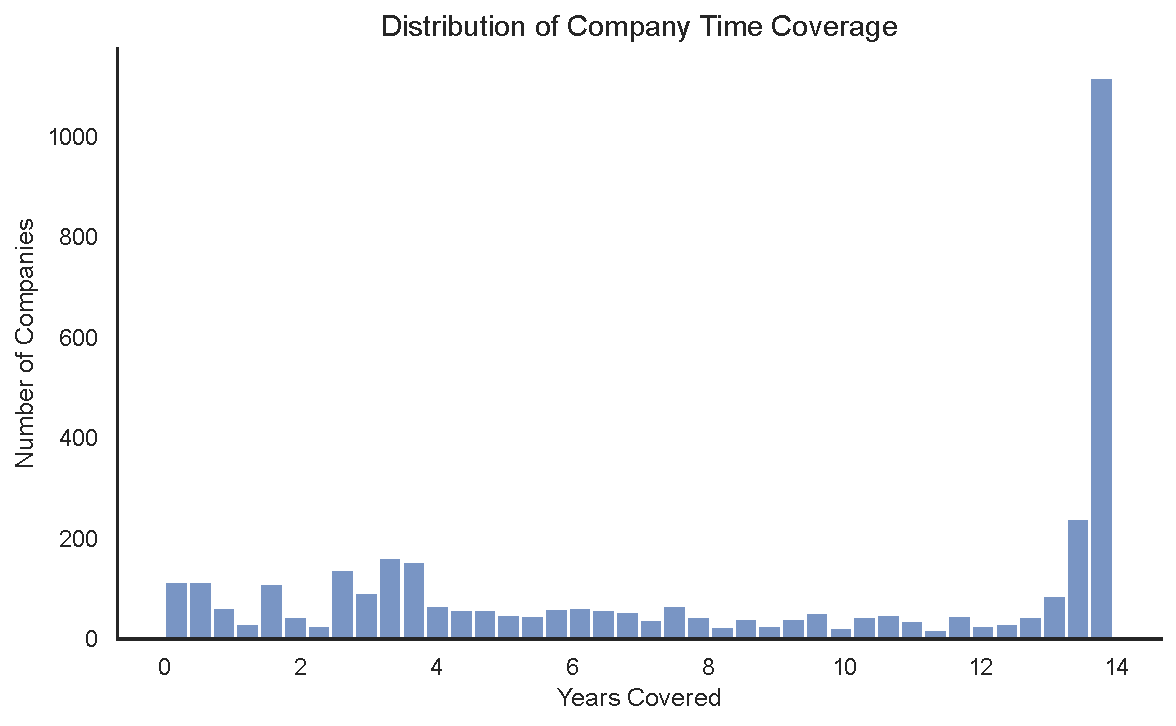
\includegraphics[width=0.75\linewidth]{sec_filings_images/company_time_coverage_distribution.pdf}
    \caption{Distribution of firm time coverage (years).}
    \label{fig:company_time_coverage}
\end{figure}

These statistics indicate that the dataset contains substantial longitudinal depth. Many firms are observed for nearly the entire sample window, while others appear for shorter periods. This structure is typical for financial panel datasets due to IPOs, delistings, mergers, and bankruptcies.

\subsection*{Panel Balance}

To evaluate the balance of the panel, we compute the standard deviation of filings per firm (19.38) and the coefficient of variation (0.59). A coefficient of variation below one indicates moderate dispersion relative to the mean.

This suggests that while firms differ in activity levels, the dataset is not extremely unbalanced. In other words, the panel is heterogeneous but not dominated by a small subset of firms with disproportionately high filing counts.

\subsection*{Implications for Downstream Modeling}

The firm-level analysis highlights several important properties of the dataset:

\begin{enumerate}
    \item \textbf{Strong cross-sectional coverage}: 3,671 firms provide a broad representation of public companies.
    \item \textbf{Meaningful longitudinal depth}: The median firm is observed for over nine years.
    \item \textbf{Low concentration}: Filing activity is not dominated by a small group of firms.
    \item \textbf{Moderate panel imbalance}: Dispersion exists but is not extreme.
\end{enumerate}

Together, these characteristics indicate that the dataset is well-suited for machine learning applications in financial text analysis. It combines sufficient firm diversity with temporal continuity, while avoiding excessive concentration that could distort model training.

\section{Sentiment Extraction}

Following section extraction and cleaning, the textual data consisted of the concatenated MD\&A and Quantitative and Qualitative Disclosures About Market Risk sections for each filing. 
In practice, the market risk section was missing in a substantial portion of the 10-Q filings and in some 10-K filings, as disclosure requirements may vary depending on firm characteristics and reporting thresholds. 
To maintain consistency across observations and avoid discarding otherwise informative samples, the extracted sections were concatenated into a single document per filing and processed jointly. 
This approach ensures that all available narrative information is utilized while preserving comparability across firms and time.

Because the objective of the study is to examine the short-term stock price impact of financial reports, particular emphasis was placed on capturing the sentiment embedded in managerial guidance and forward-looking statements. 
Prior literature suggests that tone and linguistic framing in corporate disclosures influence investor perception and subsequent returns. 
Consequently, sentiment was treated as a central textual feature.

\subsection*{BERT and FinBERT}

To extract sentiment from the textual disclosures, this study employs FinBERT\cite{yang2020finbert}, a domain-adapted transformer-based language model derived from BERT.

BERT (Bidirectional Encoder Representations from Transformers), introduced by Jacob Devlin et al. (2019)\cite{devlin2019bertpretrainingdeepbidirectional}, is based on the transformer architecture proposed by Ashish Vaswani et al. (2017)\cite{vaswani2017attention}. 
Unlike earlier sequential language models, BERT uses bidirectional self-attention mechanisms, allowing it to condition each word on both its left and right context simultaneously. 
This architecture enables deep contextual understanding of language and has become foundational in modern natural language processing.

However, general-purpose BERT models are trained on corpora such as Wikipedia and BooksCorpus, which do not reflect the specialized vocabulary and linguistic conventions of financial reporting. 
Financial text exhibits domain-specific terminology, formal structure, and nuanced expressions of uncertainty and risk that differ substantially from general language usage.

To address this limitation, FinBERT was developed as a version of BERT fine-tuned on financial corpora, including SEC filings and financial news. 
FinBERT is specifically optimized for financial sentiment classification, distinguishing between positive, negative, and neutral tone in financial contexts. 
Its training on SEC filings makes it particularly well-suited for analyzing MD\&A and related disclosure sections, as it captures the semantics and tone patterns characteristic of regulatory financial reporting.

Importantly, only the textual narrative sections extracted from the filings were used as input to FinBERT. 
Residual numerical fragments, table artifacts, and non-linguistic content were removed during preprocessing, ensuring that sentiment scores reflect meaningful narrative disclosures rather than structural noise.

\subsection*{Handling the 512-Token Limitation}

A key architectural constraint of BERT-based models is the maximum input length of 512 tokens. 
This limitation arises because the self-attention mechanism scales quadratically with sequence length in both memory and computation. 
To maintain tractability during pretraining and inference, BERT was designed with a fixed maximum positional embedding size of 512 tokens. 
Sequences exceeding this limit must therefore be truncated or segmented.

The extracted MD\&A and market risk sections frequently exceeded this limit by a substantial margin, often containing tens of thousands of tokens. 
Truncating the text to the first 512 tokens would discard potentially informative content, particularly forward-looking statements that may appear later in the section. 
Therefore, a strategy was required to approximate document-level sentiment while respecting the architectural constraint.

To address this issue, each document was divided into candidate chunks, from which a fixed number of segments were randomly sampled. 
Specifically, 48 chunks were sampled per document. 
This number was chosen based on the average character length of the filings in the dataset and computational considerations. 
It provides broad coverage of the document's content while maintaining feasible inference time given the scale of the dataset.

Each chunk was limited to 384 tokens. 
This length was selected to ensure that, after accounting for special tokens (e.g., [CLS], [SEP]) and potential padding required for batch processing, the total sequence length would not exceed the 512-token maximum. 
Using 384 tokens strikes a balance between contextual richness and computational safety, minimizing the risk of truncation while preserving meaningful semantic structure within each chunk.

Random sampling, rather than fixed sequential splitting, was adopted to avoid systematic bias toward specific portions of the document (e.g., only introductory or concluding paragraphs). 
Higher weight was given to chunks in the middle of the document, since the beginning and the end of the sections often contained boilerplate language or summary statements 
that may be less informative for sentiment analysis.
Over 48 sampled chunks, the method provides a distributed approximation of the document's overall tone.

\subsection*{Aggregation of Sentiment Scores}

FinBERT produces, for each chunk, probability scores for three sentiment categories: positive, negative, and neutral. 
To obtain document-level features representing the entire filing, these chunk-level outputs were aggregated.

For each filing, the following features were computed:
\begin{itemize}
    \item The mean positive, negative, and neutral scores across the 48 chunks.
	\item The standard deviation of the positive, negative, and neutral scores across chunks.
    \item The standard deviation of the polarity score, defined as the difference between positive and negative probabilities.
\end{itemize}

The mean sentiment scores provide an estimate of the overall tone of the disclosure, capturing whether the document is predominantly optimistic, pessimistic, or neutral in its language. 
This aligns directly with the study's objective of assessing how managerial tone influences short-term market reactions.

The standard deviations capture intra-document variability in tone. 
Financial reports may contain mixed signals—for example, strong performance in one segment and risk warnings in another. 
A high standard deviation in sentiment scores indicates heterogeneous tone across sections, which may reflect uncertainty, complexity, or conflicting information. 
Such variation may influence how investors interpret and price the disclosure.

Finally, the standard deviation of the polarity measure captures fluctuations in the balance between positive and negative language across the document. 
This feature reflects the stability or volatility of expressed sentiment and may proxy for narrative inconsistency or nuanced communication strategies.

Together, these aggregated measures transform long-form financial disclosures into compact, economically interpretable sentiment features. 
By combining domain-adapted language modeling with document-level aggregation, this approach preserves both contextual depth and cross-sectional comparability, providing structured inputs suitable for empirical analysis of short-term stock price reactions.

\subsection*{Distribution of Sentiment Features}

The results show that the predominant sentiment expressed in the reports is neutral. In particular, 
the median filing exhibits a mean neutral sentiment score above $0.8$, indicating that most sentences 
in financial disclosures are classified as neutral by the model. This observation is consistent with 
the formal and informational tone typically used in financial reporting, where companies tend to 
avoid strongly positive or negative language.

The dispersion of the sentiment scores also reveals notable patterns. The standard deviation of the 
neutral sentiment scores is often larger than that of the positive and negative scores, suggesting 
that while neutral sentiment dominates overall, the degree of neutrality varies more substantially 
across sentences within a filing. In practice, this implies that many reports contain a mixture of 
neutral statements alongside smaller portions of more opinionated or sentiment-bearing language.

Finally, the distribution of the polarity standard deviation exhibits two prominent regions, with 
many filings having values close to $0$ and another concentration around approximately $0.4$. 
Low polarity variability indicates filings in which the sentiment remains highly consistent 
throughout the document, typically reflecting uniformly neutral language. In contrast, higher 
polarity variability suggests documents where sentiment fluctuates more strongly across sections, 
potentially reflecting the coexistence of positive and negative discussions, such as descriptions 
of risks alongside favorable performance indicators.

\begin{figure}[htbp]
\centering
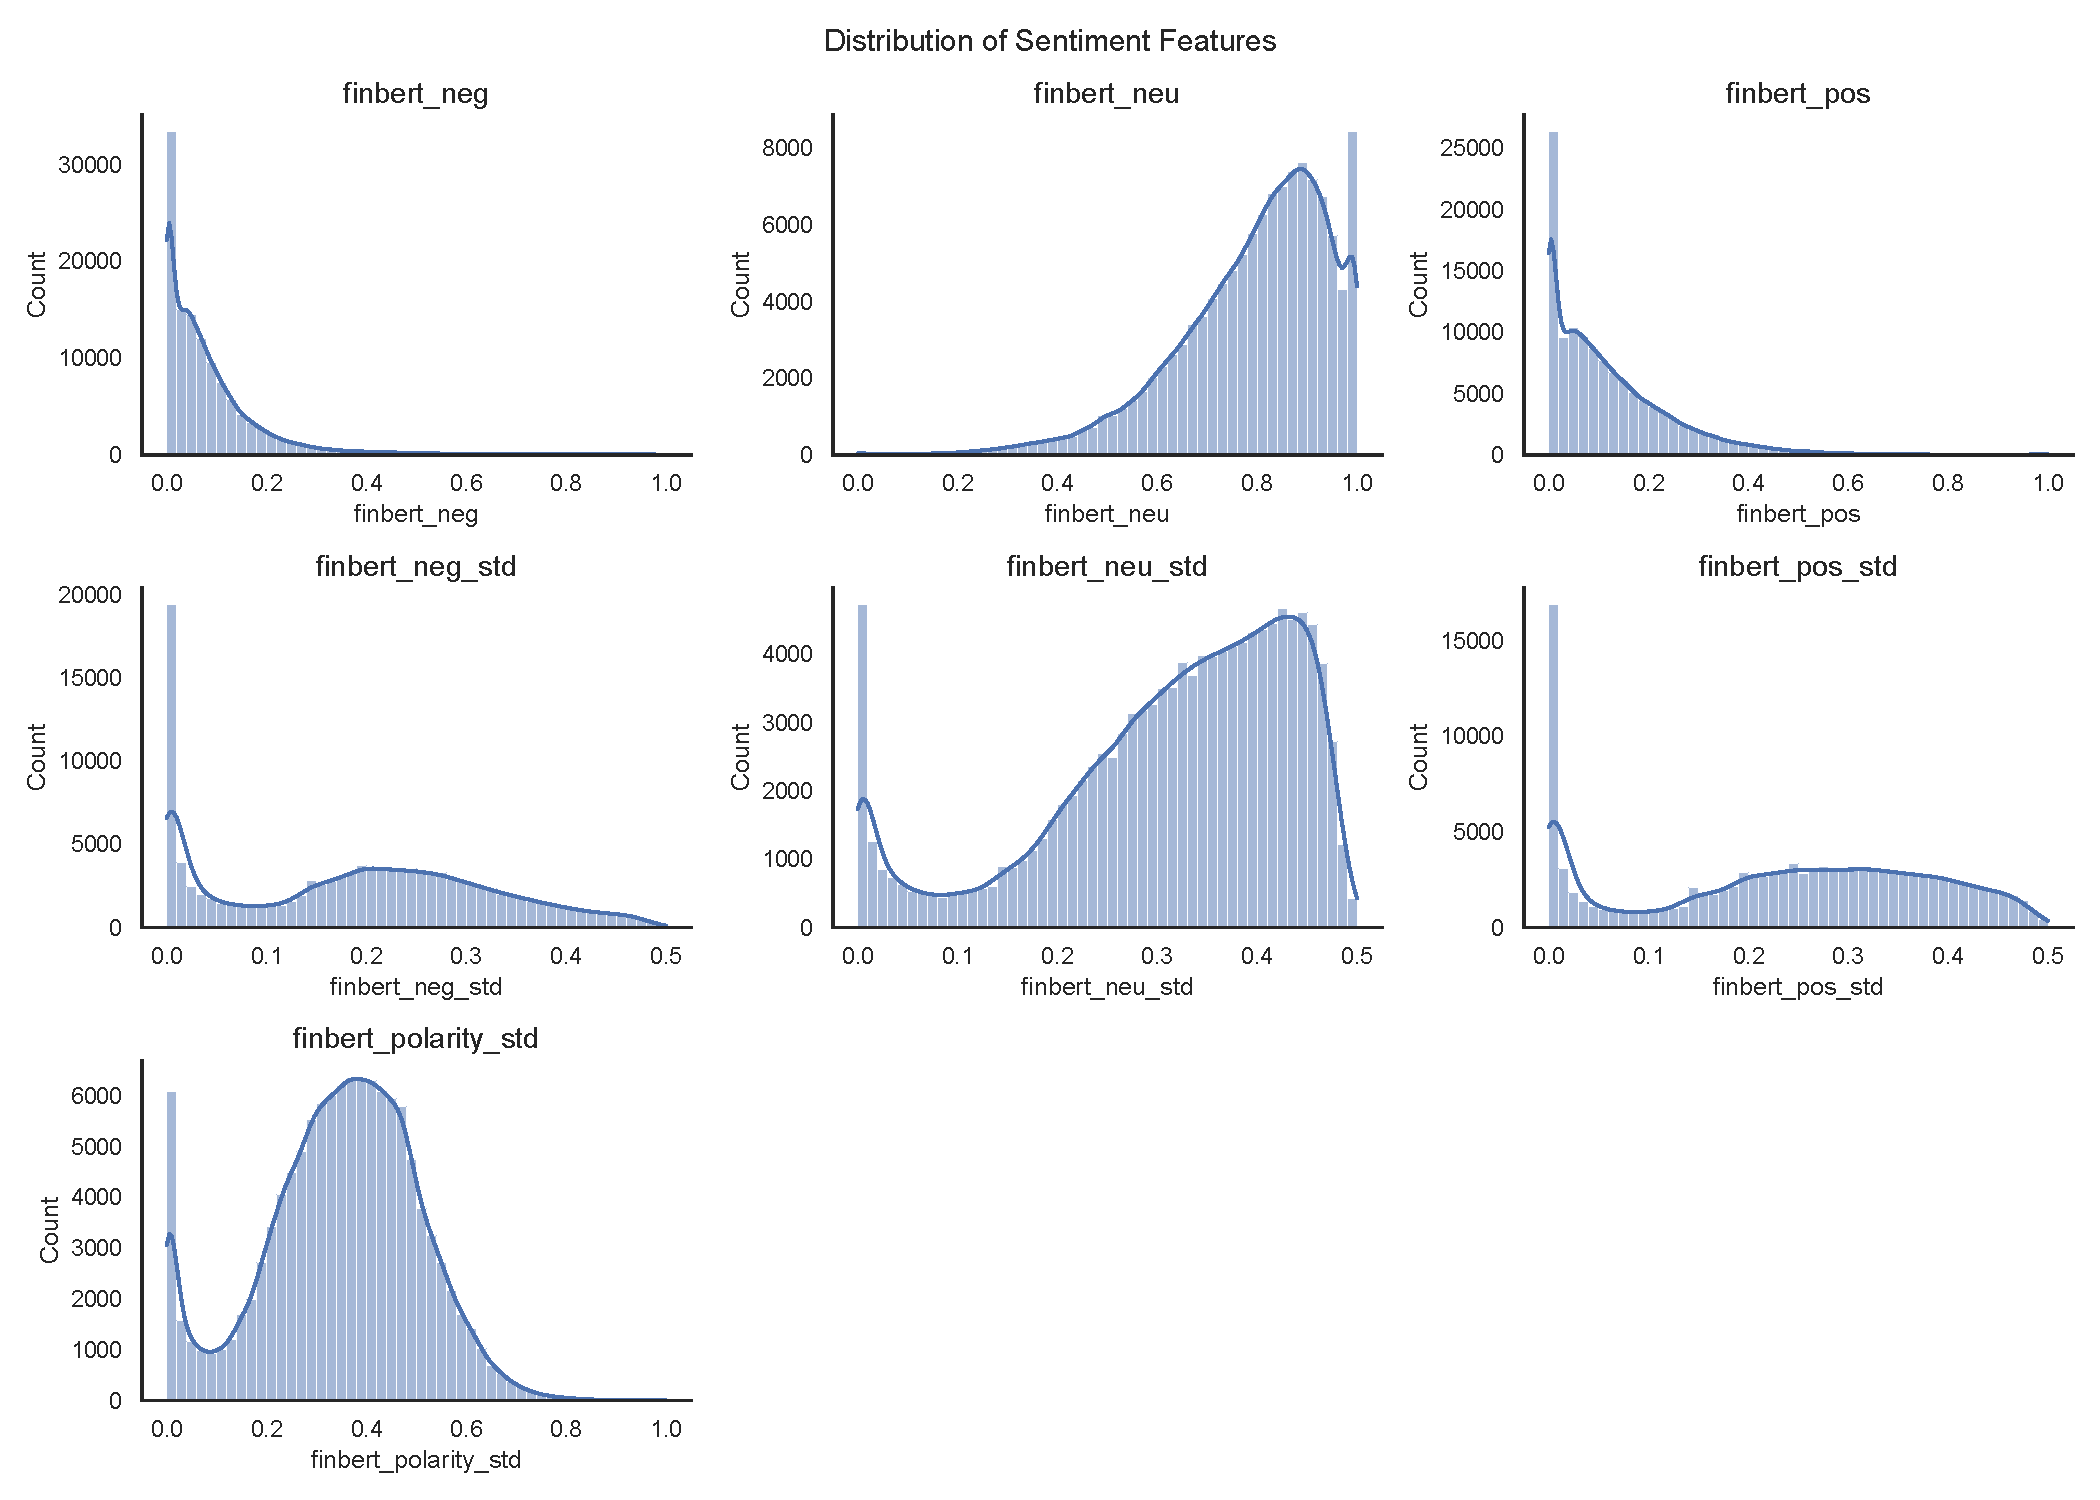
\includegraphics[width=0.9\textwidth]{sec_filings_images/sentiment_scores_distributions.pdf}
\caption{Distribution of the sentiment features extracted from financial filings using the FinBERT model.}
\label{fig:sentiment_distribution}
\end{figure}

\section{Stock Price Data}

Stock price data were obtained from \href{https://stooq.com/db/h/}{Stooq}, which provides historical daily price data for companies listed on the NYSE and NASDAQ. 
The dataset includes daily open, high, low, close, and volume information.

To align financial reports with market data, each filing was treated as an event date. 
Rather than relying solely on price information from a single day, rolling windows of preceding trading days (e.g., 5, 10, 20 days) were used to compute summary statistics such as moving averages, momentum indicators, and realized volatility measures. 
This approach compresses multiple daily observations into a single feature vector associated with each filing event. 
By incorporating recent market dynamics prior to disclosure, the dataset captures prevailing trends and risk conditions that may interact with the informational content of the filing.

\subsection{Stock Price Feature Engineering}

For each filing event occurring at trading day $t$, a lookback window of up to $L=60$ trading days prior to $t$ is used. All features are computed exclusively on observations $\{t-L, \dots, t-1\}$.

The objective of this feature construction is threefold. First, it captures prevailing market trends prior to the disclosure. Second, it summarizes recent volatility and trading activity, which may interact with the informational content of the filing. Third, it provides economically interpretable baseline indicators against which the incremental predictive value of textual sentiment can be evaluated.

\subsubsection*{Notation}

Let $P_\tau$ denote the closing price at day $\tau$, $V_\tau$ the trading volume, $H_\tau$ the daily high price, and $L_\tau$ the daily low price. Define the simple daily return as:

\begin{equation}
r_\tau = \frac{P_\tau - P_{\tau-1}}{P_{\tau-1}},
\end{equation}

for $\tau \in \{t-L+1, \dots, t-1\}$.

All statistical quantities below are computed using only the historical sample $\mathcal{H}_t = \{t-L, \dots, t-1\}$.

\subsubsection*{Last Observed Price}

The most recent closing price prior to the filing is included as:

\begin{equation}
\text{Close}_{t-1} = P_{t-1}.
\end{equation}

Although returns are scale-invariant, the price level may still contain relevant information about firm characteristics, liquidity regimes, or price clustering effects.

\subsubsection*{Moving Averages}

To capture trend dynamics, simple moving averages (SMA) are computed over multiple horizons:

\begin{equation}
\text{MA}_k(t) = \frac{1}{k} \sum_{j=1}^{k} P_{t-j},
\end{equation}

for $k \in \{5, 10, 20, 50\}$, provided sufficient historical observations exist. If fewer than $k$ observations are available, an expanding mean over the available window is used:

\begin{equation}
\text{MA}_k(t) = \frac{1}{|\mathcal{H}_t|} \sum_{\tau \in \mathcal{H}_t} P_\tau.
\end{equation}

Moving averages are widely used in technical analysis to identify short and medium-term trends. Comparing the most recent price to these averages implicitly captures momentum and mean-reversion effects.

\subsubsection*{Momentum Indicators}

Momentum measures the cumulative return over a specified lag:

\begin{equation}
\text{Momentum}_k(t) = \frac{P_{t-1}}{P_{t-1-k}} - 1,
\end{equation}

for $k \in \{5, 20\}$. If fewer than $k$ lagged observations are available, the longest feasible lag within the historical window is used.

Momentum is included because empirical finance literature documents return continuation effects over short to intermediate horizons. Pre-filing momentum may influence how new information is interpreted or priced by the market.

\subsubsection*{Volatility Measures}

Realized volatility is approximated using the sample standard deviation of daily returns. For a window of length $k$, volatility is defined as:

\begin{equation}
\sigma_k(t) = 
\sqrt{
\frac{1}{k-1}
\sum_{j=1}^{k}
\left(r_{t-j} - \bar{r}_k\right)^2
},
\end{equation}

where $\bar{r}_k$ is the mean return over the same window. Volatility is computed for $k \in \{5, 20\}$, as well as over the full available lookback window:

\begin{equation}
\sigma_{\text{full}}(t) =
\sqrt{
\frac{1}{|\mathcal{H}_t|-1}
\sum_{\tau \in \mathcal{H}_t}
\left(r_\tau - \bar{r}\right)^2
}.
\end{equation}

Short-term volatility captures immediate market uncertainty prior to the filing, while longer-window volatility reflects the broader risk regime. Elevated pre-announcement volatility may signal heightened uncertainty or information asymmetry.

\subsubsection*{Volume Standardization}

To quantify abnormal trading activity, the most recent volume is standardized relative to its historical distribution:

\begin{equation}
Z^{\text{vol}}_t =
\frac{V_{t-1} - \mu_V}{\sigma_V},
\end{equation}

where $\mu_V$ and $\sigma_V$ denote the sample mean and standard deviation of volume over $\mathcal{H}_t$. This z-score measures whether trading activity immediately prior to the filing is unusually high or low. Abnormal volume may reflect information leakage, anticipation effects, or increased investor attention.

\subsubsection*{Intraday Price Range}

Finally, the high–low range of the last historical trading day is included as a proxy for intraday volatility:

\begin{equation}
\text{HLRange}_t =
\frac{H_{t-1} - L_{t-1}}{P_{t-1}}.
\end{equation}

This normalized range captures the intensity of price fluctuations within a single day, complementing return-based volatility measures.

\subsubsection*{Economic Interpretation}

Together, these features summarize multiple dimensions of pre-filing market conditions: trend (moving averages, momentum), risk (volatility measures, high–low range), and trading activity (volume z-score). Importantly, all quantities are computed strictly before the filing date, ensuring that the predictive models operate in a realistic, forward-looking setting.

Including these structured market features serves two purposes. First, they provide a benchmark level of predictive information derived purely from price dynamics. Second, they allow for an assessment of whether textual information extracted from financial disclosures adds incremental predictive power beyond what is already embedded in historical price and volume patterns.

\section{Sector and Industry Classification}

To enrich the dataset with structural firm characteristics, sector and industry classifications were incorporated using data from the \href{https://www.nasdaq.com/market-activity/stocks/screener}{NASDAQ Stock Screener}, which provides mappings from ticker symbols to sector and industry categories. 
Including sector and industry identifiers enables cross-sectional analysis of heterogeneous effects across economic segments and allows for later examination of sector-adjusted or industry-adjusted return behavior.

\subsection*{Sector Coverage}

The dataset spans 12 unique sectors and 149 unique industries, indicating substantial economic diversity. 
The largest sectors by number of companies are Health Care, Consumer Discretionary, and Finance. In contrast, Basic Materials and Telecommunications are relatively underrepresented. This imbalance reflects broader patterns in U.S. equity markets, where certain sectors contain a larger number of publicly listed firms.

Figure~\ref{fig:companies_per_sector} visualizes the firm-level sector distribution.

\begin{figure}[H]
    \centering
    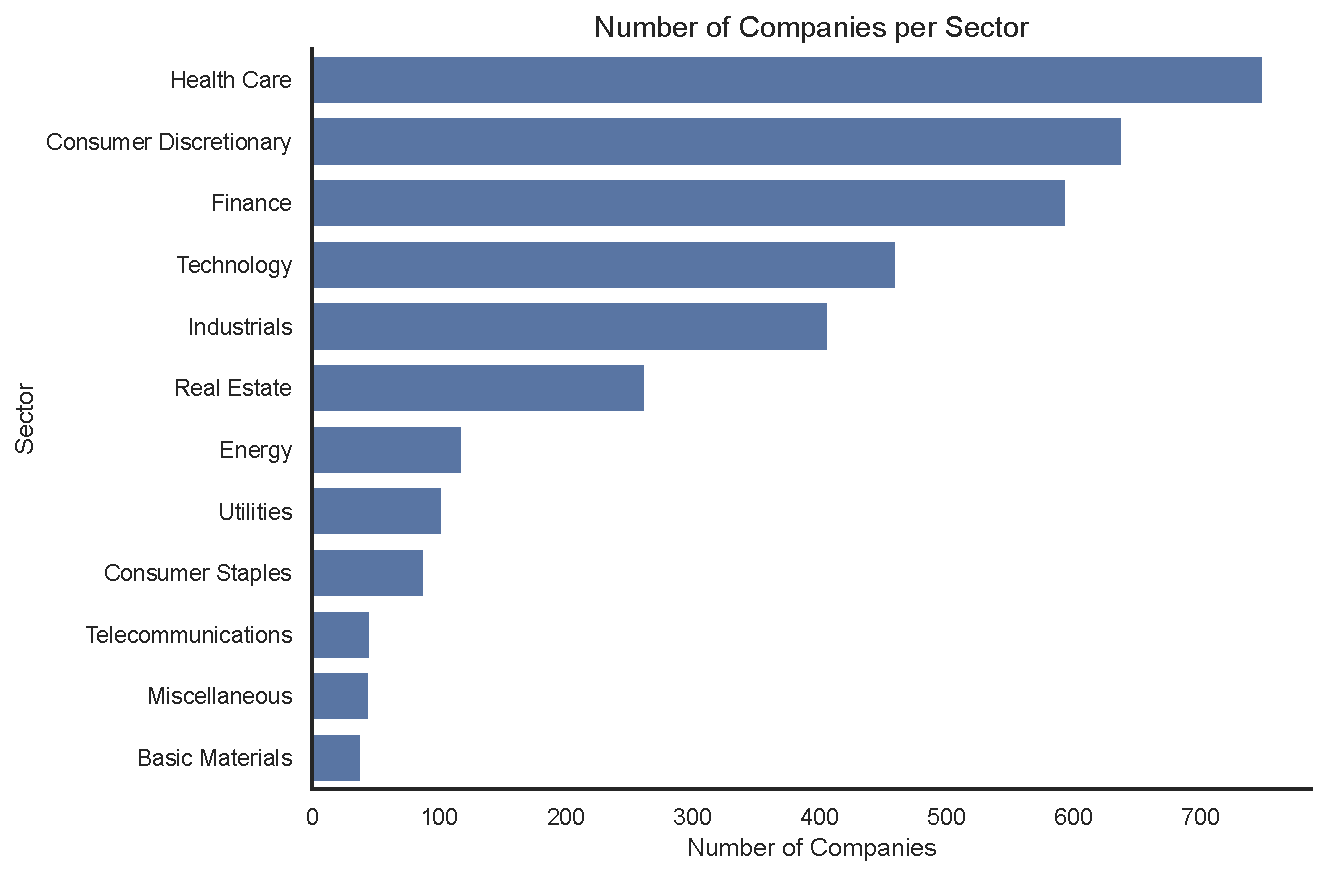
\includegraphics[width=0.8\linewidth]{sec_filings_images/companies_per_sector.pdf}
    \caption{Number of companies per sector.}
    \label{fig:companies_per_sector}
\end{figure}

When examining the distribution at the filing level, slight differences emerge.
The ordering differs somewhat from the firm-level ranking, indicating that certain sectors contribute more filings per firm on average. For example, Consumer Discretionary produces more filings than Health Care despite having fewer firms. This suggests differences in reporting intensity across sectors.

Figure~\ref{fig:filings_per_sector} illustrates the filing-level sector distribution.

\begin{figure}[H]
    \centering
    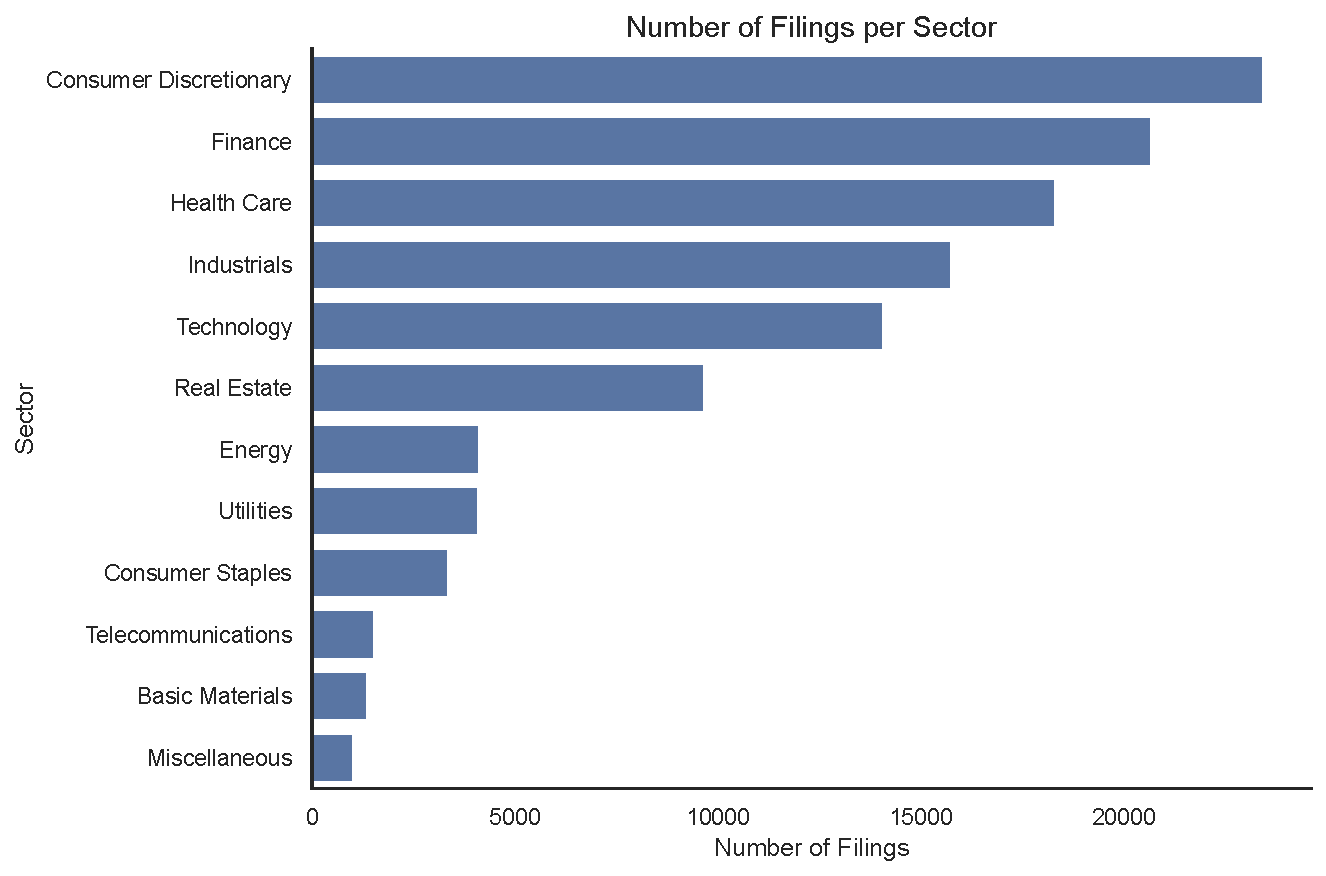
\includegraphics[width=0.8\linewidth]{sec_filings_images/filings_per_sector.pdf}
    \caption{Number of filings per sector.}
    \label{fig:filings_per_sector}
\end{figure}

From a modeling perspective, this distinction is important: sector imbalance at the firm level does not necessarily imply imbalance in the volume of textual training data. Models trained on filings may be more influenced by sectors with higher reporting intensity.

\subsection*{Industry Structure and Long-Tail Behavior}

At the industry level, the dataset contains 149 distinct industries, substantially increasing granularity relative to the 12-sector classification.
The dominance of biotechnology-related industries is particularly notable, reflecting the large number of publicly traded pharmaceutical and biotech firms.

However, the overall industry distribution exhibits a pronounced long-tail structure. The median number of companies per industry is 11, while:

\begin{itemize}
    \item 10th percentile: 3 companies
    \item 90th percentile: 45.2 companies
    \item Maximum: 364 companies
\end{itemize}

This indicates strong heterogeneity: while a few industries contain hundreds of firms, many industries are represented by only a handful of companies.

Figure~\ref{fig:top20_industries} displays the top 20 industries by firm count, while Figure~\ref{fig:industry_long_tail} visualizes the full distribution on a logarithmic scale.

\begin{figure}[H]
    \centering
    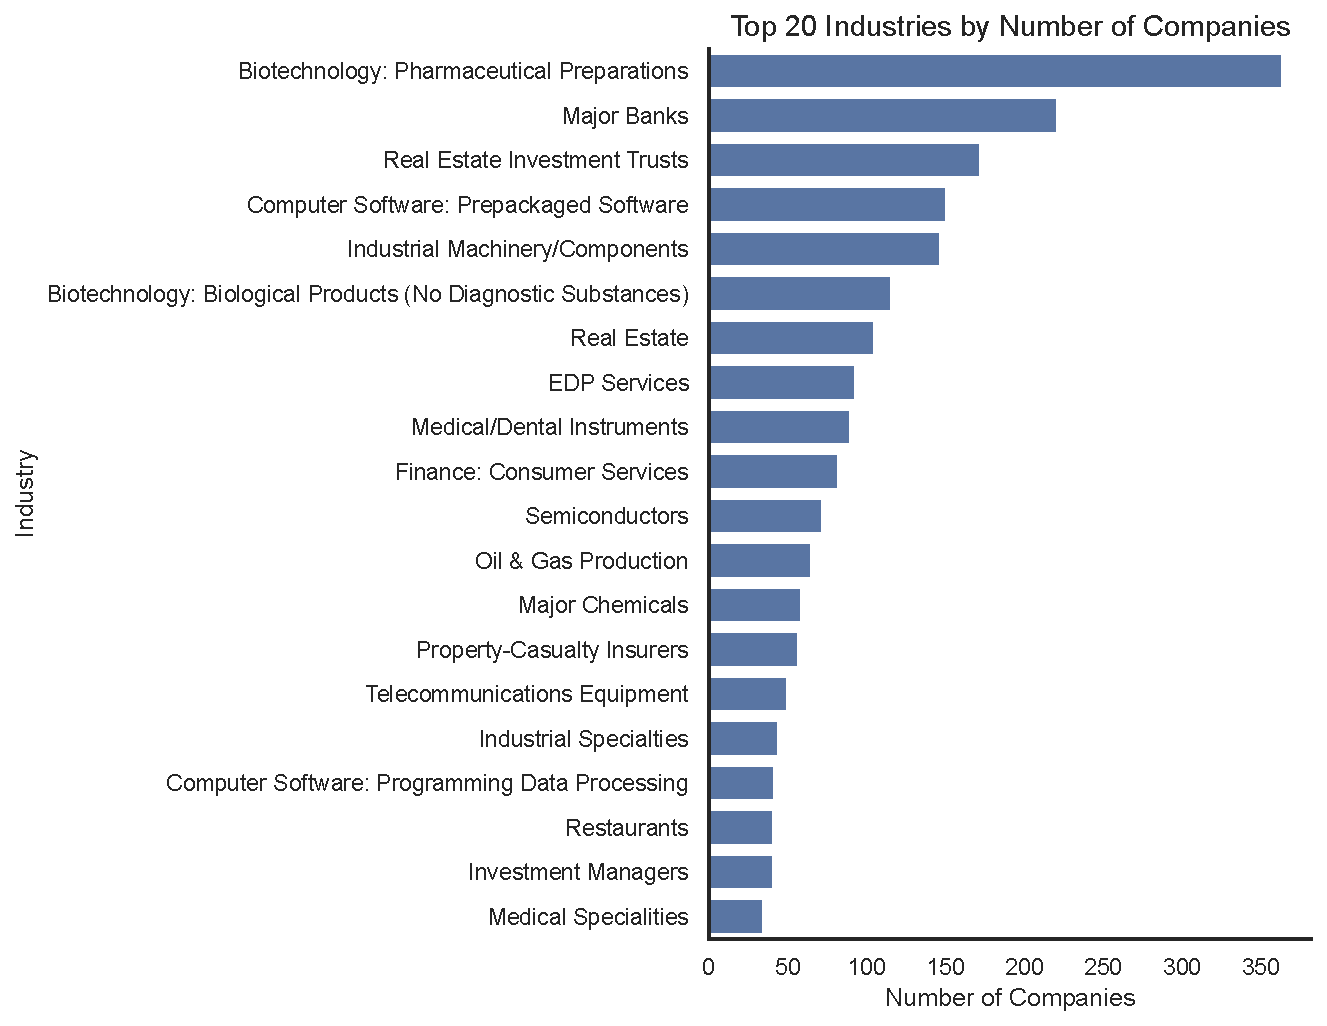
\includegraphics[width=0.85\linewidth]{sec_filings_images/top20_industries_by_companies.pdf}
    \caption{Top 20 industries by number of companies.}
    \label{fig:top20_industries}
\end{figure}

\begin{figure}[H]
    \centering
    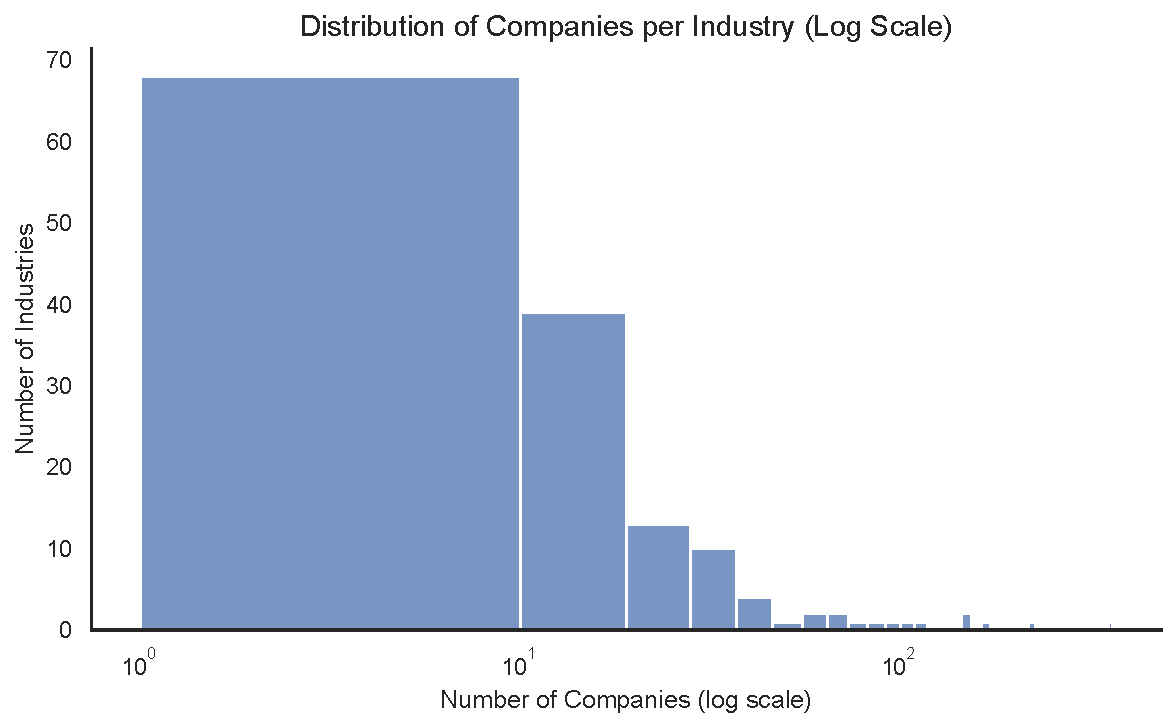
\includegraphics[width=0.75\linewidth]{sec_filings_images/industry_company_distribution_log.pdf}
    \caption{Distribution of companies per industry (log scale).}
    \label{fig:industry_long_tail}
\end{figure}

The logarithmic representation highlights the heavy-tailed nature of industry representation. Many industries contain relatively few firms, while a small number of industries dominate in terms of firm count.

\subsection*{Implications for Modeling}

The sector and industry composition of the dataset has several implications:

\begin{enumerate}
    \item \textbf{Broad economic coverage:} With 12 sectors and 149 industries, the dataset spans a wide range of economic activity.
    \item \textbf{Moderate sector imbalance:} Some sectors (e.g., Health Care, Consumer Discretionary, Finance) contain significantly more firms than others.
    \item \textbf{Industry-level fragmentation:} The industry distribution is highly skewed, with a pronounced long tail.
    \item \textbf{Potential heterogeneity in disclosure style:} Sector- and industry-specific language patterns may influence textual sentiment extraction and predictive performance.
\end{enumerate}

For machine learning applications, the long-tail industry structure implies that models may generalize well across broad sectors but could face challenges in sparsely represented industries. Conversely, the relatively balanced sector-level distribution reduces the risk that training dynamics are driven by a single economic domain.

\section{Label Construction}

Since the objective of this study is to analyze the short-term impact of financial reports on stock price dynamics, we define prediction horizons ranging from one to seven trading days following the filing date. Formally, for each filing event occurring at trading day $i$, we construct labels corresponding to horizons $h \in \{1,2,\dots,7\}$. The task is therefore to predict, based solely on information available at the filing date, the stock price movement at day $i+h$.

Both regression and classification formulations are considered. In the regression setting, we focus on relative price changes rather than absolute price levels. This choice is motivated by the substantial heterogeneity in price magnitudes across firms. Predicting absolute price differences would introduce scale distortions, as a \$1 movement has different economic meaning for a \$10 stock compared to a \$500 stock. To ensure comparability across firms, labels are defined in terms of returns.

Specifically, for each horizon $h$, the regression label is computed as the simple return:

\begin{equation}
r_{i,h} = \frac{p_{i+h} - p_i}{p_i},
\end{equation}

where $p_i$ denotes the reference price at day $i$, and $p_{i+h}$ denotes the price at day $i+h$. This formulation captures the proportional price change over the specified horizon and provides a scale-invariant measure of market reaction.

In addition to regression, a classification formulation is implemented. Inspired by the approach of Lee et al.\cite{lee-etal-2014-importance}, we define a three-class labeling scheme: \textit{UP}, \textit{STAY}, and \textit{DOWN}. A sample is labeled as:

\begin{itemize}
    \item \textit{UP} if $r_{i,h} > 0.01$,
    \item \textit{DOWN} if $r_{i,h} < -0.01$,
    \item \textit{STAY} otherwise.
\end{itemize}

The 1\% threshold is chosen to filter out minor price fluctuations that may reflect normal market noise rather than economically meaningful reactions. In highly liquid U.S. equity markets, small daily movements often arise from microstructure effects, bid-ask bounce, or general volatility. By introducing a 1\% band around zero, the classification task focuses on substantial directional moves that are more likely to reflect genuine information incorporation following earnings disclosures.

\subsubsection*{Intraday Alignment Using Filing Acceptance Time}

To more precisely capture the immediate market reaction to disclosures, we incorporate the official SEC acceptance timestamp of each filing. Earnings reports may be released before market open, during trading hours, or after market close. Ignoring this timing dimension could misalign the return calculation and dilute the measured effect.

Accordingly, the reference price $p_i$ is defined conditional on the filing time:

\begin{itemize}
    \item If the filing is published \textit{before trading hours}, the return is computed between the previous day's closing price and the same day's opening price.
    \item If the filing is published \textit{during trading hours}, the return is computed between the opening and closing price of the same trading day.
    \item If the filing is published \textit{after trading hours}, the return is computed between the same day's closing price and the next trading day's opening price.
\end{itemize}

This alignment ensures that the computed return reflects the first tradable price adjustment following public disclosure. Consequently, the constructed labels better approximate the immediate information-driven component of price movement rather than unrelated market fluctuations.

\subsubsection*{Sector and Industry Adjusted Returns}

Beyond raw returns, additional sets of labels are constructed using sector and industry adjusted returns. The motivation for this adjustment is that stock price movements are often influenced not only by firm-specific information but also by broader sectoral or industry-wide trends. For instance, macroeconomic news affecting interest rates may systematically move financial stocks, while commodity price shocks may affect energy firms collectively. In such cases, part of the observed return may reflect common factors rather than firm-specific information contained in the filing.

To isolate the idiosyncratic component of the reaction, we compute adjusted returns by subtracting the contemporaneous mean return of firms within the same sector or industry. Formally, let $\mathcal{S}(j)$ denote the set of firms belonging to the same sector (or industry) as firm $j$. The adjusted return is defined as:

\begin{equation}
\tilde{r}_{i,h}^{(j)} = r_{i,h}^{(j)} - 
\frac{1}{|\mathcal{S}(j)| - 1}
\sum_{\substack{k \in \mathcal{S}(j) \\ k \neq j}} r_{i,h}^{(k)},
\end{equation}

where a leave-one-out approach is employed to avoid mechanical bias by excluding the firm's own return from the group average. This ensures that the benchmark represents the common movement of peer firms only.

The sector and industry adjusted labels allow for a more nuanced investigation of predictive performance. If a model performs well using raw returns but poorly using adjusted returns, this may indicate that it primarily captures sector-wide trends rather than firm-specific informational effects. Conversely, strong performance on adjusted labels would suggest that the model extracts idiosyncratic signals from financial disclosures that go beyond common industry movements.

By constructing both raw and adjusted labels across multiple horizons and prediction tasks, the dataset enables a comprehensive evaluation of short-term stock price reactions to financial reports under different definitions of market response.